\documentclass[UTF8,a4paper]{ctexart}

\usepackage[a4paper,margin=2.5cm]{geometry}
\usepackage{amsmath,amssymb,amsthm}
\usepackage{graphicx}
\usepackage{booktabs}
\usepackage{array}
\usepackage{caption}
\usepackage{subcaption}
\usepackage{titlesec}
\usepackage{enumitem}
\usepackage{setspace}
\usepackage{indentfirst}
\usepackage{hyperref}
\usepackage{newtxtext,newtxmath}

% =========================================================
% 图形仿真大会中文论文骨架
% 说明：
% 1. 这是基于现有 .doc 模板与当前项目内容整理出的中文版 LaTeX 骨架。
% 2. 精确字号、页边距、行距仍需最终对照 Word 模板微调。
% 3. 推荐使用 XeLaTeX 编译；若本机缺少中文字体，可先用默认字体。
% =========================================================

\setlength{\parindent}{2em}
\setstretch{1.15}
\setlist{nosep}

% 如果本机有 Windows 中文字体，可取消注释并进一步贴近 Word 模板：
% \setCJKmainfont{SimSun}
% \setCJKsansfont{SimHei}
% \setmainfont{Times New Roman}

\captionsetup[figure]{name={图},labelsep=space,font=small}
\captionsetup[table]{name={表},labelsep=space,font=small}
\graphicspath{{figures/}{figures/crops/}}

\titleformat{\section}{\bfseries\zihao{4}}{\thesection}{0.75em}{}
\titleformat{\subsection}{\bfseries\zihao{-4}}{\thesubsection}{0.75em}{}
\titleformat{\subsubsection}{\bfseries\zihao{-4}}{\thesubsubsection}{0.75em}{}

\titlespacing*{\section}{0pt}{1.0ex plus 0.5ex minus 0.2ex}{0.8ex}
\titlespacing*{\subsection}{0pt}{0.8ex plus 0.3ex minus 0.2ex}{0.6ex}
\titlespacing*{\subsubsection}{0pt}{0.6ex plus 0.3ex minus 0.2ex}{0.4ex}

\newcommand{\papertitle}{面向稳健物体重光照的前景掩码感知相对高光引导}
\newcommand{\paperauthora}{作者甲$^{1,3}$}
\newcommand{\paperauthorb}{作者乙$^{2}$}
\newcommand{\affiliation}{
  $^{1}$单位一，城市，邮编，中国\\
  $^{2}$单位二，城市，邮编，中国\\
  $^{3}$单位三，城市，邮编，中国
}
\newcommand{\svgorpng}[2][]{%
  \includegraphics[#1]{#2.png}%
}

\begin{document}

\begin{center}
{\bfseries\zihao{3} \papertitle \par}
\vspace{1em}
{\zihao{-4} \paperauthora \qquad \paperauthorb \par}
\vspace{0.75em}
{\zihao{5} \affiliation \par}
\end{center}

\vspace{1em}

\noindent\textbf{摘要}\quad
基于扩散模型的物体重光照方法在多种照明条件下已取得较好效果，但在镜面材质、宽而软的高光波瓣以及随机面光源条件下，高光监督仍易失稳。当高光区域仅由绝对亮度阈值定义，且前景提取依赖白背景启发式规则时，这一问题尤为明显。针对上述缺陷，本文提出一种前景掩码感知的相对高光引导框架，在不增加推理复杂度的前提下提升物体重光照的稳健性。该方法优先使用显式前景掩码，仅在缺失掩码时回退到白背景阈值；在有效前景内构建局部相对亮度高光表示；基于轻微平滑后的亮度信号估计前景分位数阈值，而最终高光得分仍在原始图像域中计算；同时保留图像空间高光引导分支，以提供直接的 RGB 级监督。本文进一步构建覆盖 \textit{official}、\textit{ecommerce} 与 \textit{3D-FUTURE} 的评测协议，用于分析域内、目标域与跨域条件下的泛化能力。现有实验结果表明，所提方法能够更稳定地改善未见物体、未见环境以及随机面光源条件下的重光照质量，验证了前景感知与相对高光建模对于稳定高光监督的有效性。

\vspace{0.5em}

\noindent\textbf{关键词：}\quad
物体重光照；扩散模型；高光监督；镜面外观；跨域泛化

\section{引言}

物体重光照旨在在保持物体几何结构、材质属性与局部细节一致的前提下，合成其在新照明条件下的外观。该任务广泛应用于计算机图形学、电商内容生成与可控图像编辑等场景。近年来，扩散模型凭借强生成先验显著提升了重光照结果的真实感与稳定性，但当目标物体具有明显镜面成分，或照明条件产生宽而软的高光波瓣时，现有方法仍容易出现高光区域偏移、镜面响应失真以及边界不连续等问题。

进一步分析可发现，这类失败并不完全来自主干网络表达能力不足，而更深层地源于高光监督的构造方式。当高光区域仅依赖绝对亮度阈值确定，且前景范围由白背景启发式规则粗略估计时，背景亮区、前景裁剪误差以及条件图像中的异常光照都可能干扰监督信号。在随机面光源条件下，由于高光分布通常更宽、更软，这种不稳定性会被进一步放大。

基于上述观察，本文将研究重点放在高光监督的稳定化设计上，而非重新构造完整的重光照主干。本文提出一种前景掩码感知的相对高光引导框架：优先利用显式 alpha 或前景掩码确定有效监督区域；在有效前景内构建局部相对高光表示；仅在阈值估计阶段引入轻微高斯模糊，并通过前景内分位数估计高光阈值；在此基础上保留图像空间高光引导分支，对镜面结构相关的 RGB 细节进行直接监督。该设计不引入额外推理分支，因此能够在保持测试复杂度不变的前提下改善高光监督质量。

为充分评估所提方法，本文采用统一的 baseline 口径，并围绕标准 held-out、产品域测试和跨域测试构建实验协议。所有主结论均对齐到正确 baseline \texttt{7cn19b1e}，并在 \texttt{official}、\texttt{ecommerce} 与 \texttt{3D-FUTURE} 等不同数据划分上分析方法的稳定性与泛化能力。

本文主要贡献如下：

\begin{enumerate}
\item 识别了扩散式物体重光照在镜面材质与面光源条件下的一个关键 failure mode，即高光监督对前景分离与绝对亮度阈值高度敏感，从而导致高光区域估计不稳定。
\item 提出了一种前景掩码感知的相对高光引导框架，将前景优先掩码、局部相对高光定义、前景分位数阈值、仅用于阈值估计的模糊以及图像空间高光辅助监督有机结合。
\item 建立了区分方法消融、训练数据扩充、产品域增强与跨域测试的实验协议，为分析高光稳定性与物体重光照泛化提供了更清晰的评估框架。
\end{enumerate}

\section{相关工作}

本文与三个方向密切相关：物体重光照、基于扩散模型的条件生成，以及面向镜面高光的外观监督。

\subsection{物体重光照}

物体重光照方法旨在改变场景照明，同时保持物体身份与材质外观的一致性。早期方法通常依赖逆渲染、反射率分解或显式物理假设，这类方法虽然具有较强解释性，但往往对几何与材质估计精度高度敏感。近年来，随着生成模型的发展，重光照逐步从“显式分解再重渲染”转向“直接学习输入图像与目标光照之间的映射”。Neural Gaffer 首次系统性地展示了基于扩散模型的单图物体重光照能力，可在不进行显式场景分解的情况下，直接依据目标环境光图生成较高质量的重光照结果\cite{ref_ng}. 然而，其默认训练目标并未专门针对镜面高光监督失稳问题进行建模，这为本文的方法改进提供了空间。

\subsection{基于扩散模型的条件生成}

扩散模型在图像生成、图像编辑与条件合成任务中表现出强大的自然图像先验。相关工作已经开始探索如何为扩散模型引入更显式的光照控制。例如，LightIt 通过法线与阴影信息为扩散模型提供更明确的光照条件，从而实现更可控的照明生成与重光照\cite{ref_lightit}；SpotLight 则证明，仅利用粗略阴影提示，也能够在训练外场景中实现较细粒度的对象重光照控制\cite{ref_spotlight}。这些工作说明，扩散模型具备较强的光照理解能力，但若缺少稳定且具有针对性的监督形式，模型在高光、阴影与材质细节上的控制仍然有限。本文与上述工作不同，重点不在于引入新的控制模态，而在于重新设计高光监督本身，使其更适配镜面物体与面光源条件下的重光照训练。

\subsection{镜面与高光监督}

镜面外观建模之所以困难，是因为高光区域通常空间稀疏、形状依赖强，并且对照明变化高度敏感。对于重光照任务而言，仅依赖全局亮度阈值或简单高光 mask 容易忽略宽而软的高光波瓣，也容易受到背景高亮区域的干扰。与本文较为相关的工作包括将扩散重光照用于三维重建与多光照推断的研究。IllumiNeRF 通过先对输入图像做扩散式重光照，再重建可重光照的 NeRF，表明二维扩散重光照可以作为更复杂三维任务的重要先验\cite{ref_illuminerf}；Neural LightRig 则利用多光照扩散先验增强法线与材质估计，进一步说明多照明观测对于几何和材质恢复具有重要价值\cite{ref_lightrig}。相比之下，本文聚焦于二维物体重光照训练过程中更具体的一个问题：如何在不增加推理复杂度的前提下，提高镜面高光监督的稳定性与可解释性。为此，本文采用前景感知、前景内分位数阈值、仅用于阈值估计的模糊以及局部相对高光定义，共同构成针对该问题的监督设计。

\section{问题定义与数据协议}

本文研究条件物体重光照问题。给定输入物体图像 $x$、目标照明条件 $c$ 以及目标重光照图像 $y$，模型学习映射
\begin{equation}
\hat{y} = f_{\theta}(x, c),
\end{equation}
其中 $\hat{y}$ 应在保持物体身份与几何结构的同时匹配目标照明外观。

\subsection{高光监督失稳问题}

本文关注的核心问题是扩散式物体重光照中的一个重复出现的 failure mode：

\begin{enumerate}
\item 高光监督对前景与背景分离高度敏感；
\item 绝对亮度阈值在宽而软的高光波瓣下不稳定；
\item 条件图像中异常光照会干扰高光估计；
\item 随机面光源划分比常规划分更容易暴露这一问题。
\end{enumerate}

\subsection{符号定义}

记 $M \in \{0,1\}^{H \times W}$ 为前景掩码，$I$ 为图像，$B(\cdot)$ 为仅用于阈值估计的轻量高斯模糊算子。记 $Q_q(\cdot)$ 为在有效前景像素内计算的 $q$ 分位数。训练过程中，重光照模型在前景区域上同时受到重建损失与高光相关损失约束。

\subsection{数据协议}

根据当前项目规划，训练与评估分为以下几个阶段：

\begin{enumerate}
\item \textbf{方法消融：} 使用 \texttt{official-1000}，用于所有核心方法消融及与正确 baseline 的公平比较。
\item \textbf{主模型扩展：} 使用 \texttt{official-1000 + official-2000}，验证方法在更大但同分布数据上是否仍然成立。
\item \textbf{产品域增强：} 在主模型基础上引入 \texttt{ecommerce-1000}，通过 balanced mix 或 finetune 方式分析目标域增强效果。
\item \textbf{跨域测试：} 使用 \texttt{3D-FUTURE} held-out 测试，优先作为 test-only benchmark，而非一开始就加入主训练集。
\end{enumerate}

为保证结论一致性，本文所有关键结果均应锚定到正确 baseline \texttt{7cn19b1e}。

\section{方法}

本文方法的目标是在不增加推理阶段复杂度的前提下稳定高光监督。整体框架包含五个核心部分：前景优先掩码、相对高光定义、基于分位数的阈值估计、仅用于阈值估计的模糊，以及图像空间高光引导。

\subsection{整体流程}

整个训练流程可以概括为：

\begin{enumerate}
\item 优先从显式 alpha 或前景 mask 中提取可靠的前景支持区域；
\item 在有效前景内计算局部相对高光度量；
\item 在轻微平滑后的信号上、仅针对前景像素估计稳定阈值；
\item 在不替代原始 RGB 监督的前提下构造图像空间高光引导目标；
\item 联合优化扩散重光照主目标与高光相关辅助目标。
\end{enumerate}

\begin{figure}[htbp]
\centering
\svgorpng[width=\linewidth]{figures/neural_gaffer_highlight_model}
\caption{基于当前代码结构的高光感知 Neural Gaffer 训练框架示意图。}
\label{fig:model_arch_cn}
\end{figure}

\subsection{前景掩码感知监督}

当数据中存在显式 alpha 或分割 mask 时，本文优先使用这些前景信息；仅当显式 mask 缺失时，才回退到白背景阈值规则。这样可以显著减少背景高亮区域被误判为高光的风险。

记 $M$ 为有效前景掩码，则所有高光统计都仅在满足 $M=1$ 的像素上计算。

\begin{equation}
M(p)=
\begin{cases}
1, & \text{若显式 alpha 或 mask 将 } p \text{ 标记为前景},\\
\mathbb{I}\!\left(\min\nolimits_c I_c(p) < \tau_{\text{bg}}\right), & \text{否则},
\end{cases}
\end{equation}
其中 $\tau_{\text{bg}}$ 表示白背景回退阈值。

\subsection{相对高光定义}

不同于仅依赖绝对亮度的高光定义，本文在有效前景内构建局部相对高光表示，以强调相对局部背景更亮的区域。其一般形式可写为
\begin{equation}
S_{\text{rel}}(p) = \phi\big(I(p), \mathcal{N}(p), M\big),
\end{equation}
其中 $p$ 为像素位置，$\mathcal{N}(p)$ 表示局部邻域，$\phi$ 刻画局部相对亮度差异。

\begin{figure}[htbp]
\centering
\svgorpng[width=\linewidth]{figures/local_relative_highlight_comparison}
\caption{全局绝对亮度阈值与局部相对高光检测的对比示意图。}
\label{fig:relative_cmp_cn}
\end{figure}

在当前实现中，本文采用前景归一化的局部差分形式：
\begin{equation}
\mu_{\text{fg}}(p)=
\frac{\sum_{q \in \mathcal{N}(p)} M(q)\,L(q)}
{\sum_{q \in \mathcal{N}(p)} M(q)+\varepsilon},
\qquad
S_{\text{rel}}(p)=L(p)-\mu_{\text{fg}}(p),
\end{equation}
其中 $L$ 表示亮度图，$\varepsilon$ 为数值稳定项。

\subsection{前景内分位数阈值}

高光阈值仅由有效前景像素估计：
\begin{equation}
\tau = Q_q \big( \{ B(I(p)) \mid M(p)=1 \} \big),
\end{equation}
其中 $q$ 为前景分位数。这样可以避免背景像素扭曲阈值估计，并增强不同物体类别之间的稳定性。

\subsection{仅用于阈值估计的模糊}

为增强高光区域的空间连贯性，本文仅在阈值估计阶段对亮度图做轻微高斯模糊：

\begin{equation}
\tilde{I} = B(I), \qquad \tau = Q_q(\tilde{I} \odot M).
\end{equation}

最终高光得分仍然基于原始图像亮度计算，而不是直接在模糊图上计算，从而保留细粒度高光边界。

\begin{equation}
T(p)=
\begin{cases}
\tau, & \text{绝对模式},\\
\mu_{\text{fg}}(p)+\tau, & \text{差分模式},
\end{cases}
\end{equation}
其中 $T(p)$ 表示还原到亮度域后的最终阈值图。

\begin{equation}
H(p)=
\left(
\frac{\max\left(L(p)-T(p), 0\right)}
{\max\left(1-T(p), \epsilon\right)}
\right)^\gamma
\cdot M(p),
\end{equation}
其中 $H$ 为软高光得分图，$\gamma$ 为软权重指数。

\begin{figure}[htbp]
\centering
\svgorpng[width=\linewidth]{figures/highlight_supervision_flow}
\caption{前景掩码感知相对高光监督流程示意图。}
\label{fig:hl_flow_cn}
\end{figure}

\subsection{图像空间高光引导}

在标准重光照目标之外，本文保留图像空间高光引导分支，以直接约束 RGB 域中的高光结构。与纯 latent replacement 相比，这一分支能够提供更高信息量的监督信号，因此更适合作为主方法主线。

当启用效率变体时，本文还训练一个轻量 latent probe，以从预测 clean latent 中直接回归相同的高光分数：
\begin{equation}
\hat{H}_{\text{latent}} = P_\psi(\hat{z}_0),
\end{equation}
其中 $\hat{z}_0$ 表示预测的 clean latent，$P_\psi$ 表示 latent highlight probe。

\subsection{训练目标}

整体目标函数写为
\begin{equation}
\mathcal{L} = \lambda_{\text{rec}}\mathcal{L}_{\text{rec}} + \lambda_{\text{perc}}\mathcal{L}_{\text{perc}} + \lambda_{\text{hl}}\mathcal{L}_{\text{highlight}}.
\end{equation}

\begin{equation}
\mathcal{L}_{\text{rec}} = \| (\hat{y} - y) \odot M \|_1.
\end{equation}

\begin{equation}
\mathcal{L}_{\text{highlight}} = \| G(\hat{y}, M) - G(y, M) \|_1,
\end{equation}
其中 $G(\cdot)$ 表示前景掩码感知的相对高光引导算子。

\begin{equation}
\mathcal{L}_{\text{probe}}=
\text{BCE}\!\left(\hat{H}_{\text{latent}}, H(y)\right).
\end{equation}

对于 hybrid probe distillation 设置，训练目标可写为
\begin{equation}
\mathcal{L}_{\text{hybrid}}=
\mathcal{L}_{\text{diff}}
\,+\,\alpha(t)\mathcal{L}_{\text{highlight}}
\,+\,\beta(t)\mathcal{L}_{\text{probe}},
\end{equation}
其中 $\alpha(t)$ 随训练步数逐步衰减图像空间高光分支权重，$\beta(t)$ 则逐步提高 probe 分支权重。

\section{实验}

\subsection{实验目标}

本文实验主要回答以下四个问题：

\begin{enumerate}
\item 主方法是否优于正确 baseline，并提升高光监督稳定性？
\item 各模块对最终性能提升的贡献分别是什么？
\item 当训练数据扩充到更大规模或迁移到产品域时，方法收益是否依然保持？
\item 该方法在 \texttt{3D-FUTURE} 等未见域上是否仍具有泛化能力？
\end{enumerate}

\subsection{实现细节}

所有对比均基于 \texttt{train\_neural\_gaffer\_highlight\_gpu1} 项目中的统一配置展开，主 baseline 为 \texttt{7cn19b1e}。模型主干继承自 Neural Gaffer 的二维扩散重光照框架，其条件输入由物体图像 latent、HDR 环境光图 latent 与 LDR 环境光图 latent 共同构成，并在通道维与噪声 latent 拼接后送入 U-Net 进行去噪预测。训练过程中使用 $256\times256$ 分辨率，评价指标包括 PSNR、SSIM、LPIPS，以及 \texttt{uu}、\texttt{us}、\texttt{ra}、\texttt{tu} 和 \texttt{train} 五个划分上的重光照指标。

在当前主方法配置中，前景掩码优先由显式 mask 提供，白背景阈值回退参数设为 \texttt{0.96}；高光分位数阈值采用 \texttt{q=0.88}；仅用于阈值估计的高斯模糊参数设置为 $\sigma=1.0$；局部相对高光使用 difference 模式，局部窗口大小为 \texttt{15}；随机光照条件采样概率设为 \texttt{0.4}。图像空间高光辅助分支与高光权重均使用 warmup 策略，以减小训练早期高光监督过强带来的不稳定性。

\subsection{基于现有证据的阶段性消融表}

当前仓库中尚未为每一个模块都补齐严格单因素、同预算的 clean ablation。因而表 \ref{tab:evidence_ablation_cn} 记录的是与代码演化过程对齐的阶段性证据，而不是最终投稿版的严格消融。

\begin{table}[htbp]
\centering
\small
\setlength{\tabcolsep}{3.8pt}
\caption{基于 \texttt{official-1000} 的现有证据对齐版消融结果}
\label{tab:evidence_ablation_cn}
\begin{tabular}{p{3.9cm}ccccccc}
\toprule
方法变体 & uu & us & ra & tu & Avg. & Delta & train \\
\midrule
原始正确 baseline（\texttt{7cn19b1e}） & 31.1904 & 30.1492 & 28.3970 & 29.5503 & 29.8217 & +0.0000 & 28.4476 \\
+ 图像空间高光引导，固定阈值（\texttt{qju56ygl}） & 30.0675 & 29.3631 & 26.5557 & 30.0620 & 29.0121 & -0.8097 & 30.0214 \\
+ 分位数阈值 + 随机光照条件（\texttt{nsniycxi}） & 30.7810 & 29.5849 & 25.4691 & 29.6327 & 28.8669 & -0.9548 & 27.6715 \\
+ \texttt{q=0.88} + 前景回退清理（\texttt{jbhdfvfc}） & \textbf{31.7993} & 30.6854 & 28.4180 & 28.9659 & 29.9672 & +0.1454 & \textbf{30.4835} \\
+ 仅用于阈值估计的模糊（\texttt{spuru5qy}） & 31.6393 & \textbf{30.7137} & \textbf{28.9569} & 28.8678 & \textbf{30.0444} & \textbf{+0.2227} & 28.9013 \\
+ 局部相对高光定义（\texttt{fi04f78e}） & 31.4897 & 30.4535 & 28.0178 & 29.4746 & 29.8589 & +0.0372 & 28.6971 \\
\bottomrule
\end{tabular}
\end{table}

\noindent\textbf{说明：} 上表为当前可直接写入论文初稿的阶段性证据表。其中 \texttt{Avg.} 表示 \texttt{uu/us/ra/tu} 四个 held-out 指标的平均值，\texttt{Delta} 表示相对于正确 baseline 的平均增益。正式投稿前仍建议补充同训练预算、单变量控制的 clean ablation，以分别验证前景优先、blur-only threshold estimation 与 local-relative highlight 的独立贡献。

\subsection{主力结果参考}

\begin{table}[htbp]
\centering
\caption{当前 corrected baseline 协议下的代表性 run}
\begin{tabular}{lccccc}
\toprule
Run & uu & us & ra & tu & train \\
\midrule
\texttt{7cn19b1e} baseline & 31.1904 & 30.1492 & 28.3970 & 29.5503 & 28.4476 \\
\texttt{jbhdfvfc} 主 held-out 最强 run & 31.7993 & 30.6854 & 28.4180 & 28.9659 & 30.4835 \\
\texttt{spuru5qy} 最均衡 run & 31.6393 & 30.7137 & 28.9569 & 28.8678 & 28.9013 \\
\texttt{fi04f78e} 相对高光主线 run & 31.4897 & 30.4535 & 28.0178 & 29.4746 & 28.6971 \\
\bottomrule
\end{tabular}
\end{table}

\subsection{阶段性结果分析}

从当前 corrected baseline 协议下的已有 run 可见，本文方法主线已经形成较为明确的性能增益趋势。与正确 baseline \texttt{7cn19b1e} 相比，\texttt{jbhdfvfc} 在 \texttt{uu} 上提升至 \texttt{31.7993}，相对增益为 \texttt{+0.6089}，同时在 \texttt{us} 与 \texttt{train} 上分别达到 \texttt{30.6854} 与 \texttt{30.4835}。该结果说明，当高光监督由固定阈值逐步过渡到前景感知、自适应分位数和图像空间高光辅助约束时，模型在主要 held-out 设置上能够获得稳定增益。

进一步地，\texttt{spuru5qy} 在 \texttt{ra} 上达到 \texttt{28.9569}，表现出当前最好的随机面光源鲁棒性。与较早的 \texttt{nsniycxi} 相比，其 \texttt{ra} 提升了 \texttt{3.4878}，说明仅依赖分位数阈值仍不足以充分覆盖宽而软的面光源高光，而 blur-only threshold estimation 能够有效增强高光区域的空间连贯性，从而改善该划分下的监督质量。

另一方面，\texttt{fi04f78e} 在引入 local relative highlight 后，\texttt{uu} 与 \texttt{us} 仍保持在较高水平，说明相对亮度建模在不显著牺牲主指标的情况下，提高了方法的可解释性与高光定义的合理性。尽管其单项指标尚未全面超过 \texttt{jbhdfvfc} 或 \texttt{spuru5qy}，但它为本文方法的公式化表述与原理分析提供了最直接的实验支撑。

综合来看，前景感知、前景内分位数阈值、仅用于阈值估计的模糊以及局部相对高光定义共同构成了当前最可信的主方法路线。其中，\texttt{jbhdfvfc} 更适合作为主方法锚点，\texttt{spuru5qy} 更适合作为随机面光源鲁棒性的补充证据，而 \texttt{fi04f78e} 则更适合作为方法原理与消融解释的代表 run。

\subsection{训练数据策略}

第二组实验用于区分“方法收益”与“数据扩充收益”。

\begin{table}[htbp]
\centering
\small
\setlength{\tabcolsep}{4pt}
\caption{训练数据策略比较}
\begin{tabular}{p{4.6cm}ccc}
\toprule
训练协议 & Official Held-out & Ecommerce Held-out & 3D-FUTURE Held-out \\
\midrule
\texttt{official-1000} & TBD & TBD & TBD \\
\texttt{official-1000 + official-2000} & TBD & TBD & TBD \\
\texttt{official + official\_2000 + ecommerce} balanced mix & TBD & TBD & TBD \\
主模型 $\rightarrow$ \texttt{ecommerce} finetune & TBD & TBD & TBD \\
\bottomrule
\end{tabular}
\end{table}

\subsection{跨域泛化}

第三组实验用于验证主方法是否可以迁移到未见数据域。

\begin{table}[htbp]
\centering
\caption{official、ecommerce 与 3D-FUTURE 上的跨域泛化结果}
\begin{tabular}{lccc}
\toprule
方法 & official & ecommerce & 3D-FUTURE \\
\midrule
Baseline & TBD & TBD & TBD \\
完整主方法 & TBD & TBD & TBD \\
Hybrid probe distillation & TBD & TBD & TBD \\
Pure latent probe replacement & TBD & TBD & TBD \\
\bottomrule
\end{tabular}
\end{table}

\subsection{效率变体}

probe 系列方法在论文中应作为效率变体呈现，而不应与主方法混为一体。

\begin{table}[htbp]
\centering
\caption{主方法与效率变体的效果-效率对比}
\begin{tabular}{lccccc}
\toprule
方法 & Peak VRAM & Steps/hour & uu & us & ra \\
\midrule
图像空间主方法（\texttt{fi04f78e}） & TBD & TBD & 31.4897 & 30.4535 & 28.0178 \\
Hybrid probe distillation（\texttt{xkmlb19f}） & TBD & TBD & 30.9751 & 29.5747 & \textbf{29.2093} \\
Pure latent replacement（\texttt{iepfybfu}） & TBD & TBD & 30.0771 & 27.6759 & 29.0589 \\
\bottomrule
\end{tabular}
\end{table}

\subsection{效率变体分析}

从效率变体结果来看，\texttt{xkmlb19f} 与 \texttt{iepfybfu} 不宜作为主方法主线，但为本文提供了有价值的效果-效率权衡证据。\texttt{xkmlb19f} 在 \texttt{ra} 上达到当前最优的 \texttt{29.2093}，说明 hybrid probe distillation 能够在随机面光源条件下保留较强的高光建模能力；然而其 \texttt{uu} 与 \texttt{us} 仍低于主方法锚点 run，因此更适合作为辅助效率版本，而非核心贡献。

相比之下，\texttt{iepfybfu} 作为 pure latent replacement，虽然在 \texttt{ra} 上同样达到较高水平，但其 \texttt{uu} 和 \texttt{us} 明显回落，尤其 \texttt{us} 仅为 \texttt{27.6759}。这表明若完全以 latent probe 替代图像空间高光分支，虽然可能降低训练代价，却会削弱主 held-out 设置下的性能表现。

因此，本文更合理的写作策略是：将 image-space 主方法作为效果主线，将 hybrid probe distillation 作为减轻 decode-backprop 依赖的效率增强候选，而将 pure latent replacement 作为验证图像空间高光分支必要性的负对照实验。

\subsection{定性结果展示}

根据当前规划，正文中至少应包含以下几类图示：

\begin{enumerate}
\item 原始 baseline 在 area-light 与 soft highlight 条件下的失败案例；
\item 方法整体流程图；
\item official held-out 中 \texttt{uu}、\texttt{us}、\texttt{ra} 的可视化对比；
\item \texttt{official}、\texttt{ecommerce}、\texttt{3D-FUTURE} 的跨域可视化对比；
\item image-space、hybrid 与 pure probe 的效果-效率对照图。
\end{enumerate}

\subsection{定性结果分析与图示组织原则}

从当前 \texttt{wandb/media} 中的结果图来看，已有若干样例足以支撑论文初稿中的问题定义图、主对比图与效率图。首先，随机面光源划分中的若干样例已经明显展示出本文方法在宽而软高光条件下的优势。以 \texttt{jbhdfvfc} 和 \texttt{spuru5qy} 的 \texttt{unseen\_object\_with\_random\_area\_light\_condition} 面板为例，模型输出能够更接近目标图像的镜面明暗分布，并减少过度追随输入条件图像外观的问题。

其次，\texttt{unseen\_object\_with\_unseen\_envir} 与 \texttt{unseen\_object\_with\_seen\_envir} 中的一些样例能够较好地展示本文方法在主 held-out 任务上的一致性提升。这类图更适合作为正文主图，用于支撑“方法并非只在随机面光源上有效，而是在主测试协议上整体提升”的结论。

再次，当前训练日志里已经保存了高光 mask 与高光 weight 图。这些图虽然不适合作为主结果图，但非常适合放在方法诊断图中，用于展示本文高光定义从“绝对亮度阈值”转向“前景感知、分位数与相对高光”之后的监督形态。

\begin{figure}[htbp]
\centering
\begin{subfigure}{0.68\linewidth}
\centering
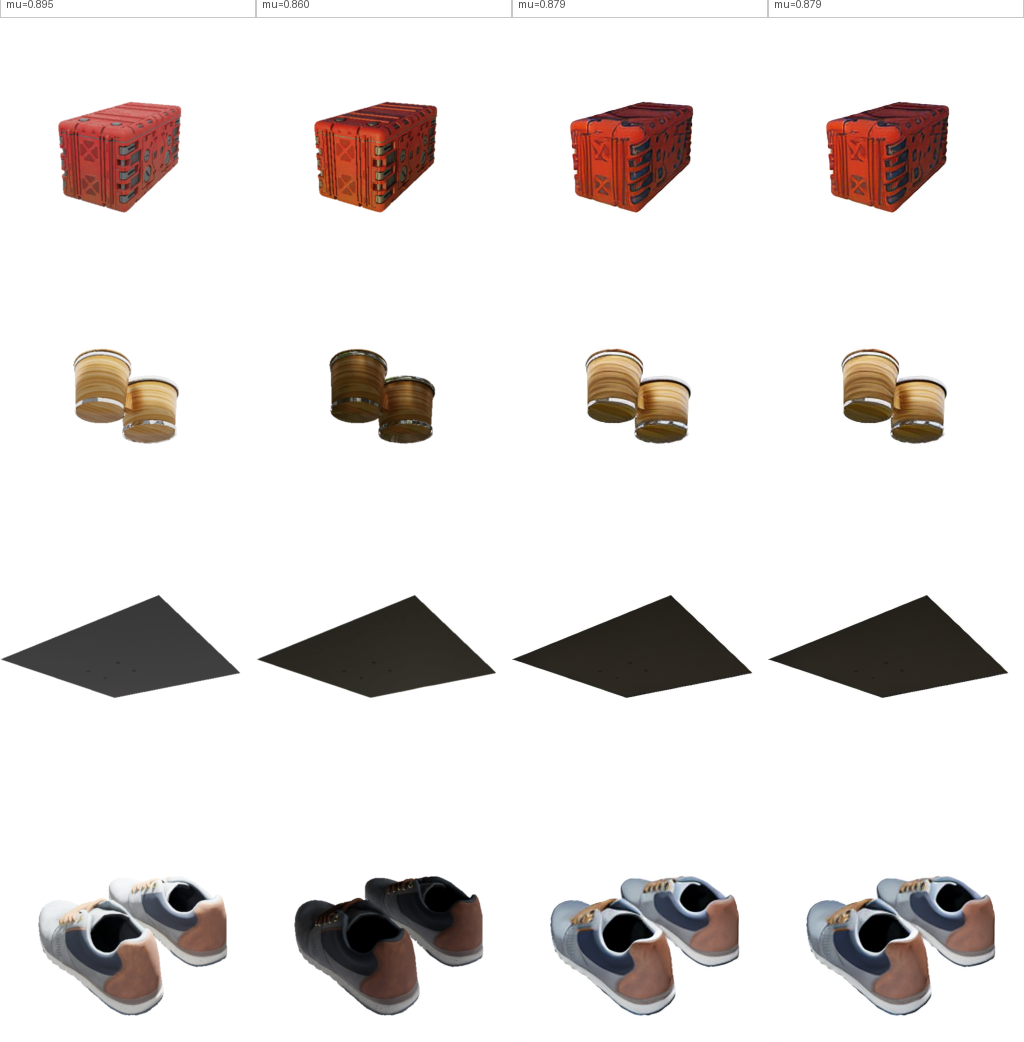
\includegraphics[width=\linewidth]{problem_def_ra_failure_result.png}
\caption{随机面光源失败样例结果区}
\end{subfigure}\hfill
\begin{subfigure}{0.28\linewidth}
\centering
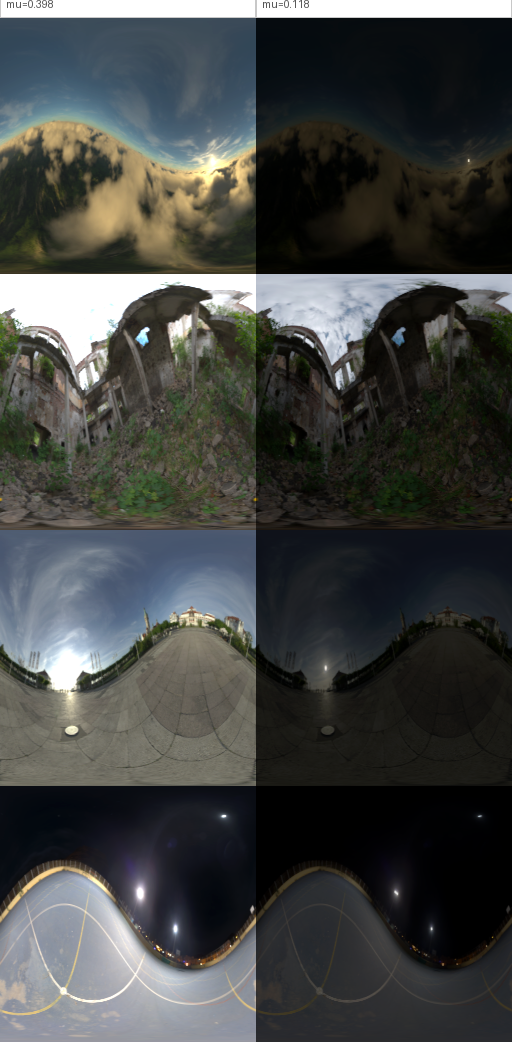
\includegraphics[width=\linewidth]{problem_def_ra_failure_env.png}
\caption{对应照明条件}
\end{subfigure}
\caption{问题定义图。早期分位数高光版本在随机面光源与宽波瓣高光条件下仍存在明显失稳现象，说明仅依赖绝对亮度或粗糙阈值策略不足以稳定高光监督。}
\label{fig:problem_def_cn}
\end{figure}

\begin{figure}[htbp]
\centering
\svgorpng[width=\linewidth]{figures/highlight_supervision_flow}
\caption{方法流程图。图中展示了前景优先掩码、局部相对高光计算、blur-only threshold estimation 与图像空间高光引导之间的关系。}
\label{fig:method_flow_cn}
\end{figure}

\begin{figure}[htbp]
\centering
\begin{subfigure}{0.32\linewidth}
\centering
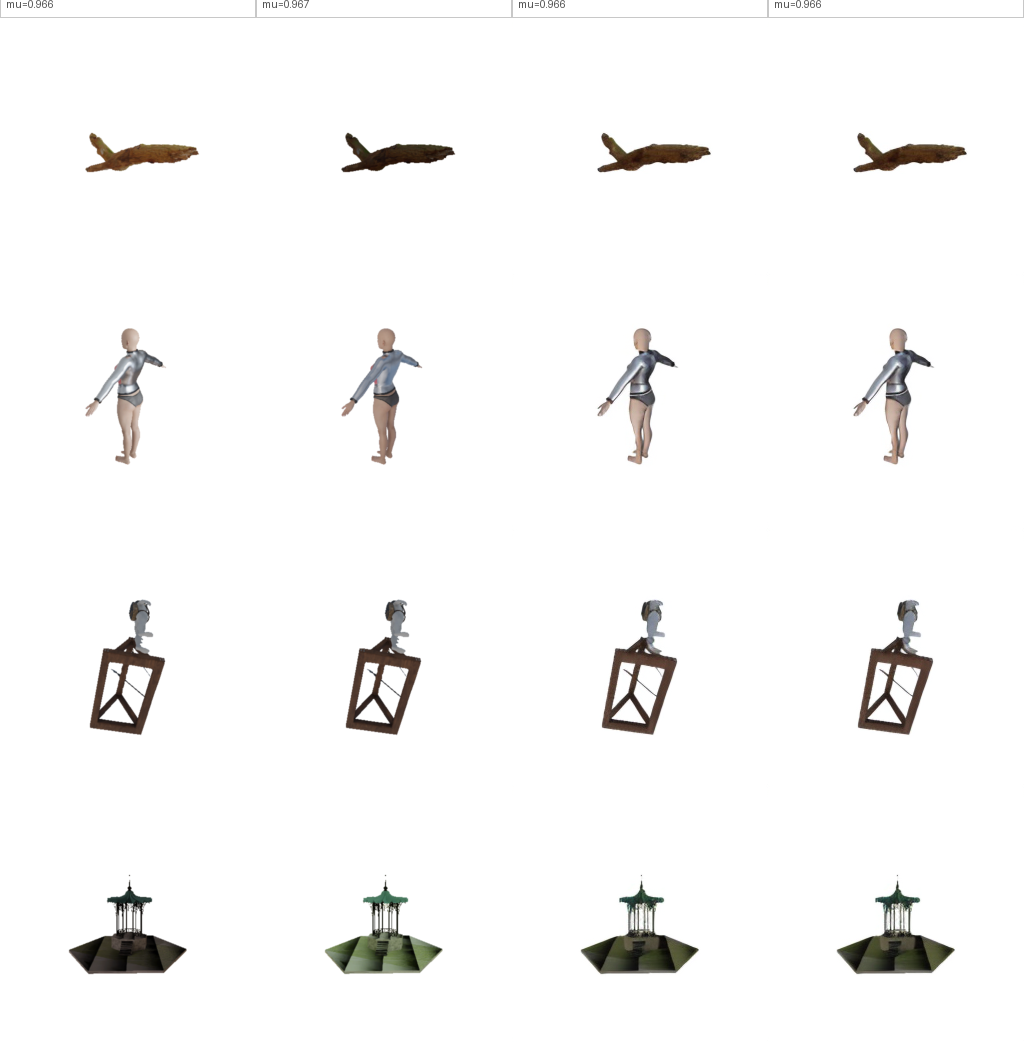
\includegraphics[width=\linewidth]{official_uu_main_result.png}
\caption{\texttt{uu}}
\end{subfigure}\hfill
\begin{subfigure}{0.32\linewidth}
\centering
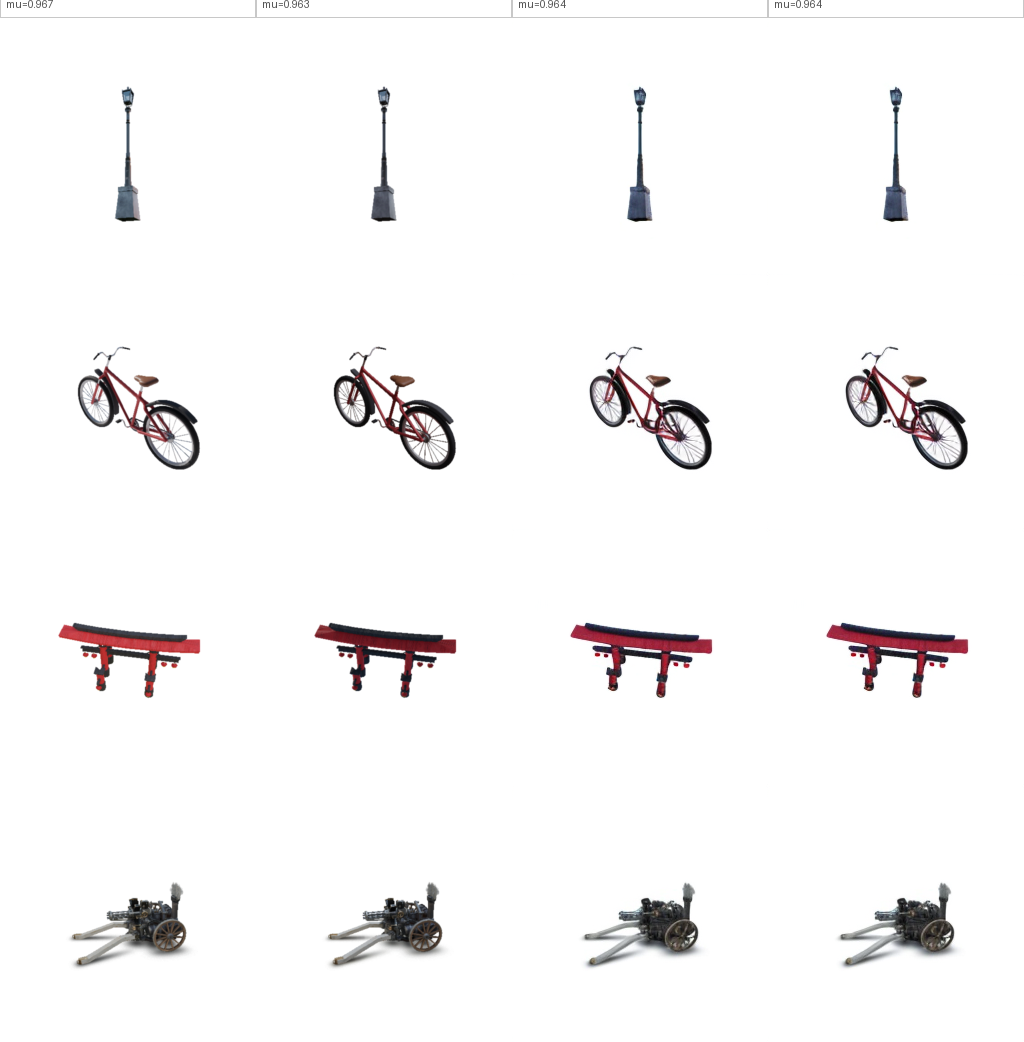
\includegraphics[width=\linewidth]{official_us_main_result.png}
\caption{\texttt{us}}
\end{subfigure}\hfill
\begin{subfigure}{0.32\linewidth}
\centering
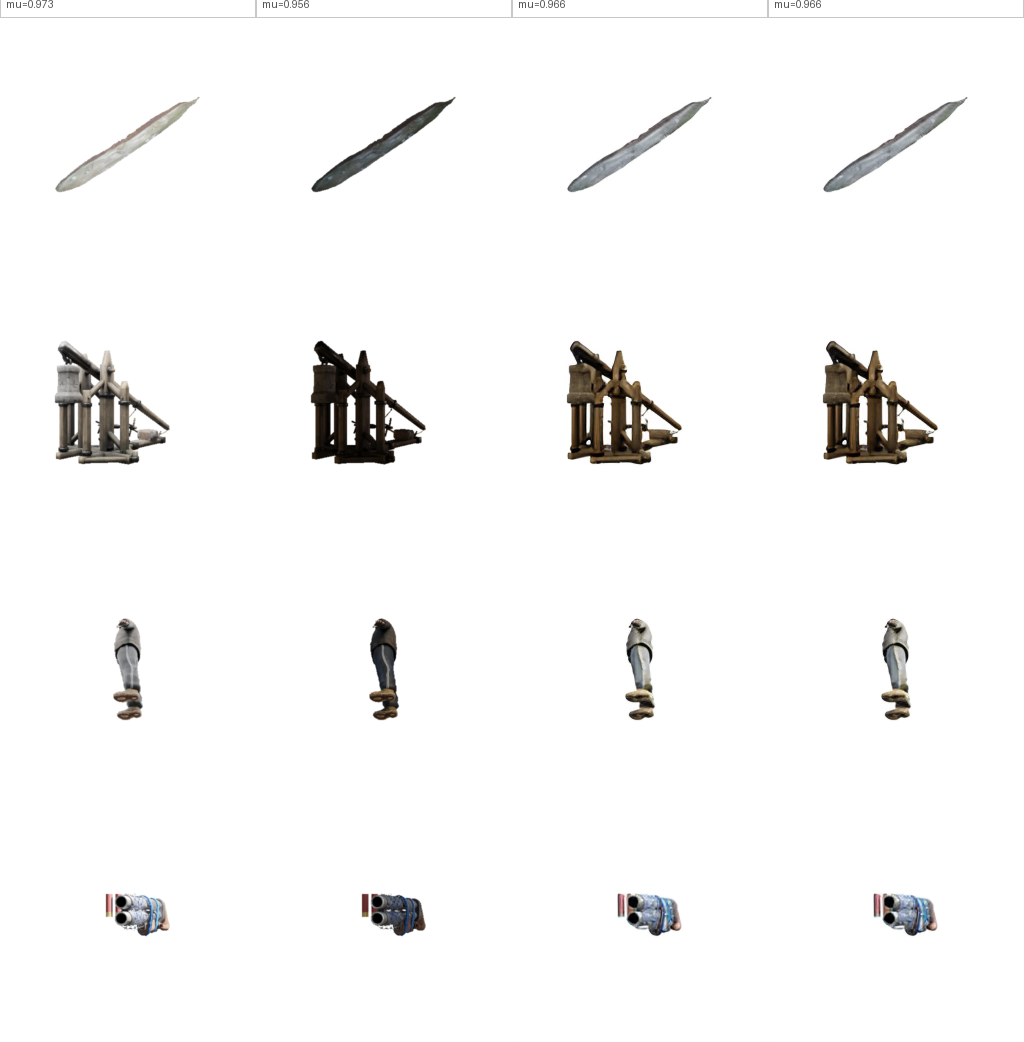
\includegraphics[width=\linewidth]{official_ra_main_result.png}
\caption{\texttt{ra}}
\end{subfigure}
\caption{official held-out 结果裁图。三种划分下，本文方法均能较稳定地匹配目标照明外观；其中 \texttt{ra} 更能体现方法在宽而软高光条件下对镜面区域的改善。}
\label{fig:official_main_cn}
\end{figure}

\begin{figure}[htbp]
\centering
\fbox{\rule{0pt}{5.0cm}\rule{0.92\linewidth}{0pt}}
\caption{跨域对比图占位。预留 \texttt{official}、\texttt{ecommerce} 与 \texttt{3D-FUTURE} 三列，每列展示 baseline、本文方法与局部高光放大图。}
\end{figure}

\begin{figure}[htbp]
\centering
\begin{subfigure}{0.32\linewidth}
\centering
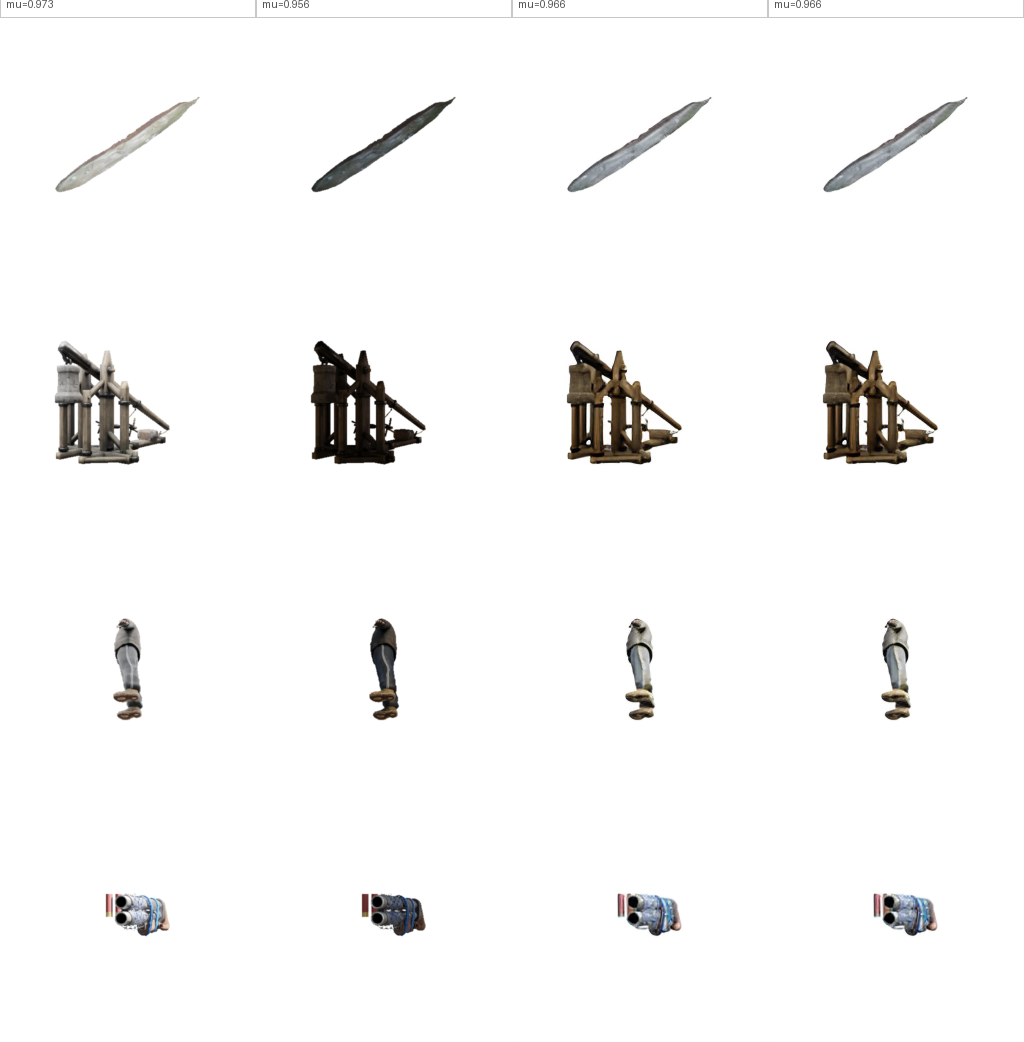
\includegraphics[width=\linewidth]{official_ra_main_result.png}
\caption{image-space 主方法}
\end{subfigure}\hfill
\begin{subfigure}{0.32\linewidth}
\centering
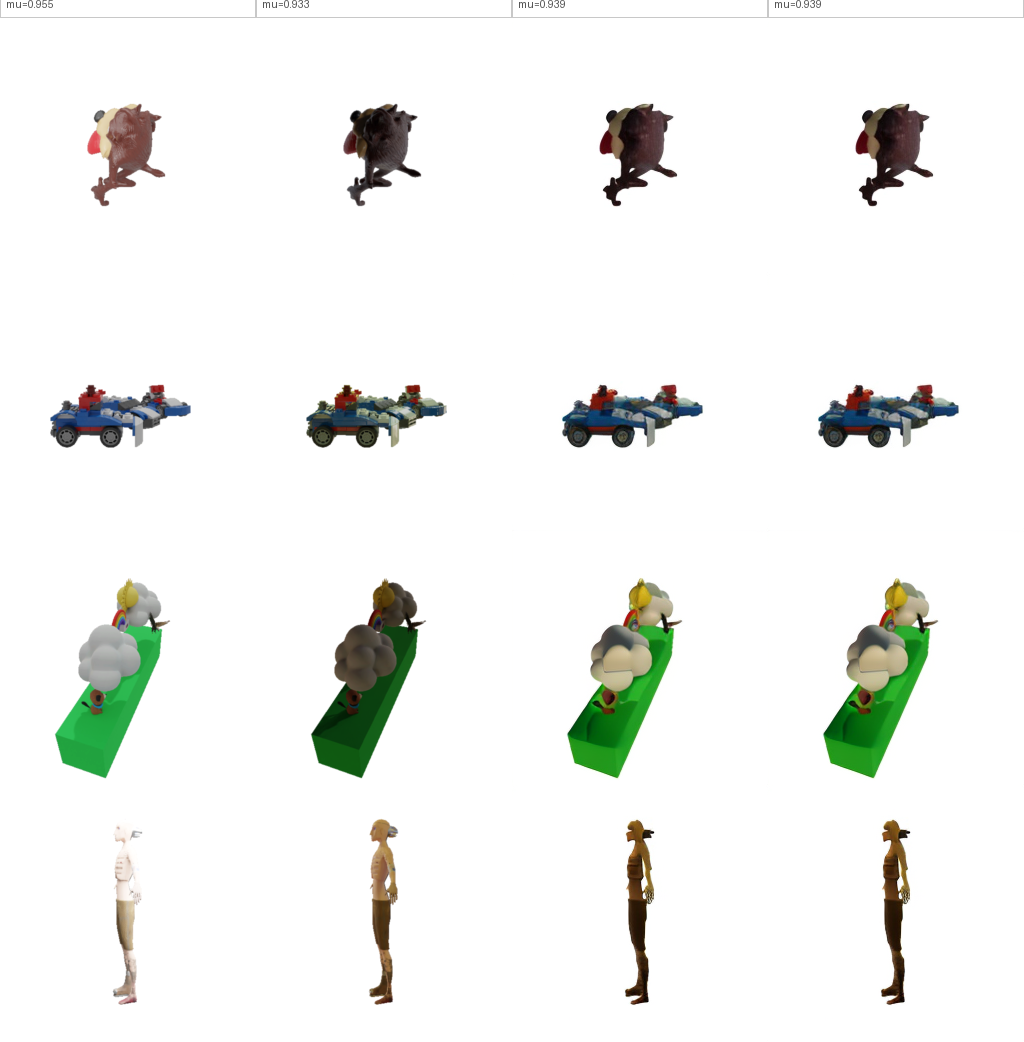
\includegraphics[width=\linewidth]{efficiency_hybrid_ra_result.png}
\caption{hybrid probe distillation}
\end{subfigure}\hfill
\begin{subfigure}{0.32\linewidth}
\centering
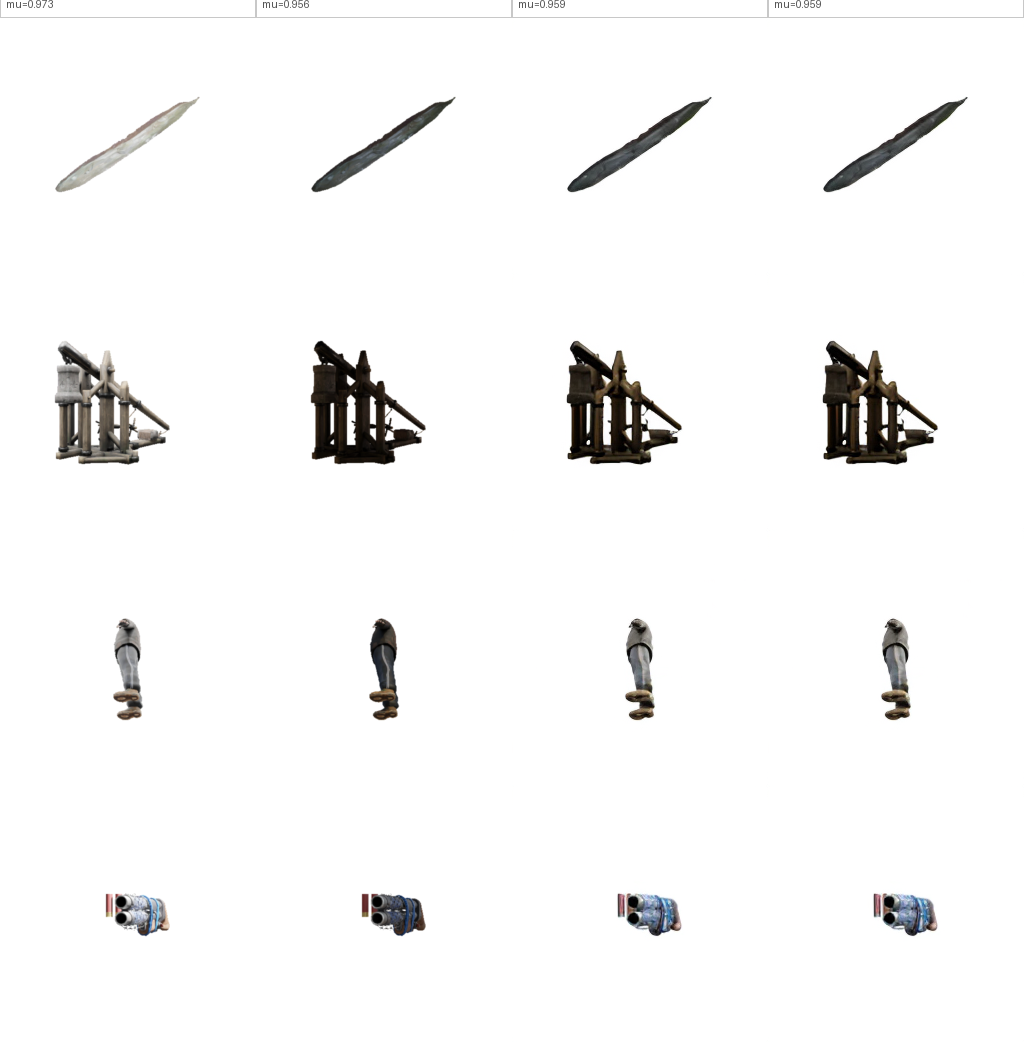
\includegraphics[width=\linewidth]{efficiency_replacement_ra_result.png}
\caption{pure latent replacement}
\end{subfigure}
\caption{效果-效率对比图。三种设置在随机面光源条件下的结果均能维持基本可用的高光外观，但 hybrid probe distillation 在保持较强 \texttt{ra} 表现的同时，更适合作为效果与效率折中的辅助方案。}
\label{fig:efficiency_vis_cn}
\end{figure}

\begin{figure}[htbp]
\centering
\begin{subfigure}{0.32\linewidth}
\centering
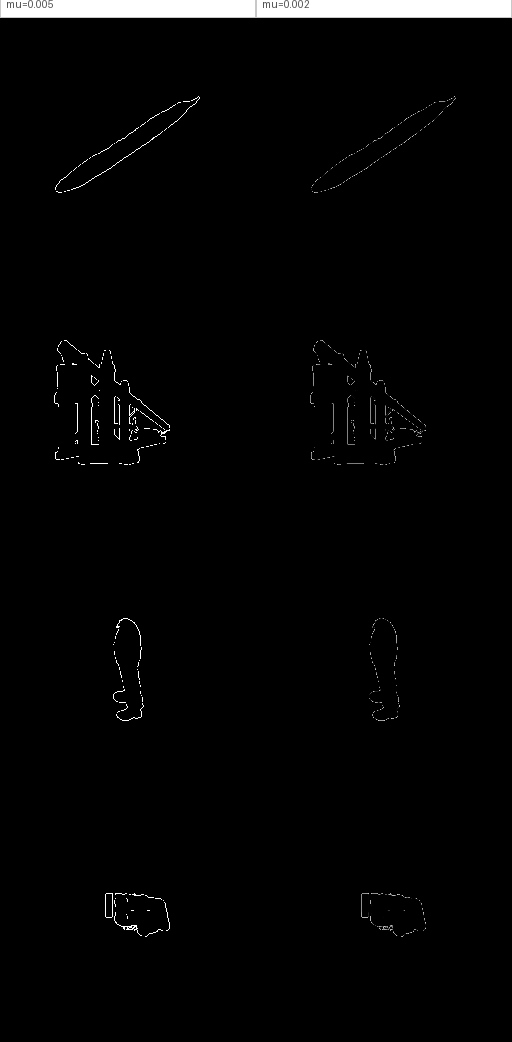
\includegraphics[width=\linewidth]{official_ra_main_diagnostic.png}
\caption{结果面板中的诊断区域}
\end{subfigure}\hfill
\begin{subfigure}{0.15\linewidth}
\centering
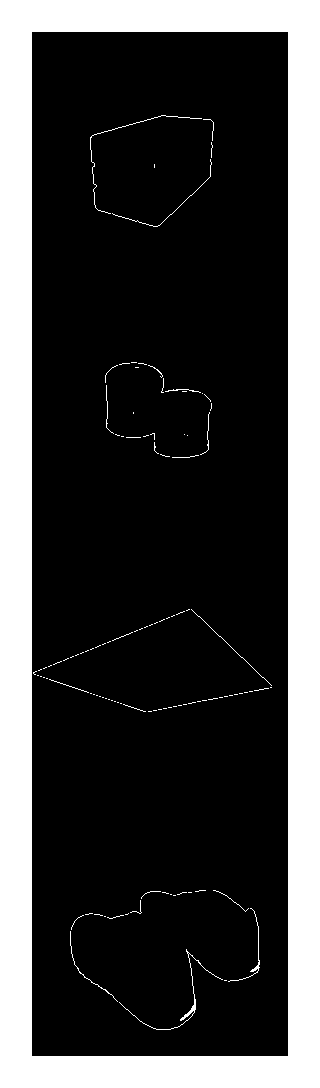
\includegraphics[width=\linewidth]{official_ra_mask.png}
\caption{高光 mask}
\end{subfigure}\hfill
\begin{subfigure}{0.15\linewidth}
\centering
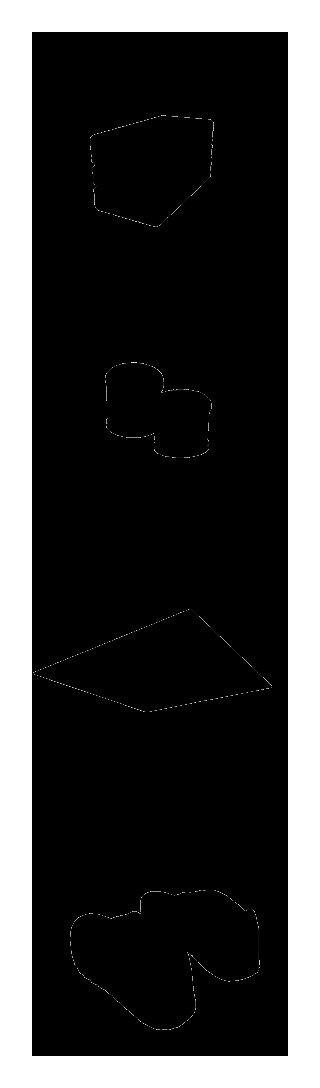
\includegraphics[width=\linewidth]{official_ra_weight.png}
\caption{高光 weight}
\end{subfigure}\hfill
\begin{subfigure}{0.32\linewidth}
\centering
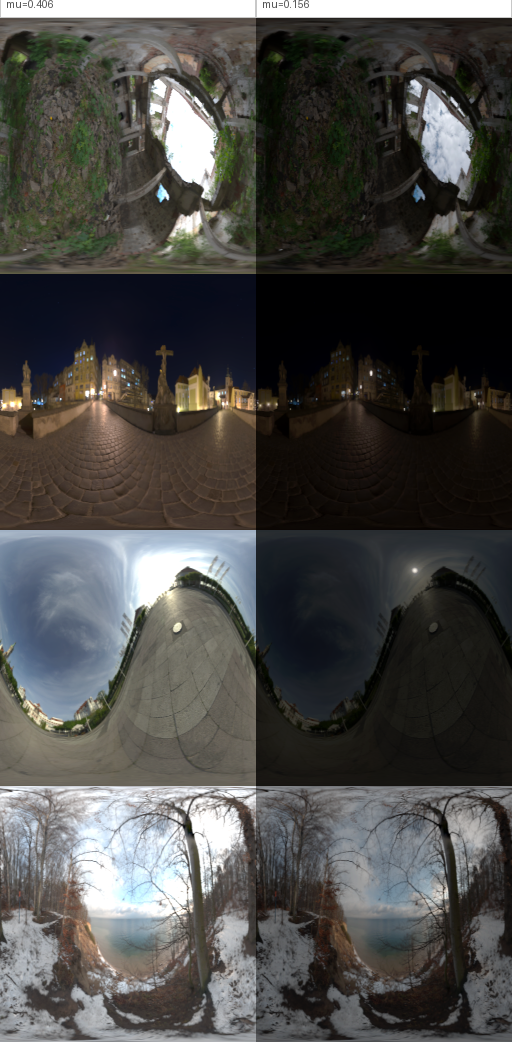
\includegraphics[width=\linewidth]{official_ra_main_env.png}
\caption{HDR/LDR 环境图}
\end{subfigure}
\caption{方法诊断图。前景感知高光监督不仅约束结果图像，还通过高光 mask、soft weight 与目标环境图共同提供更稳定的训练信号。}
\label{fig:diagnostic_cn}
\end{figure}

\begin{figure}[htbp]
\centering
\begin{subfigure}{0.68\linewidth}
\centering
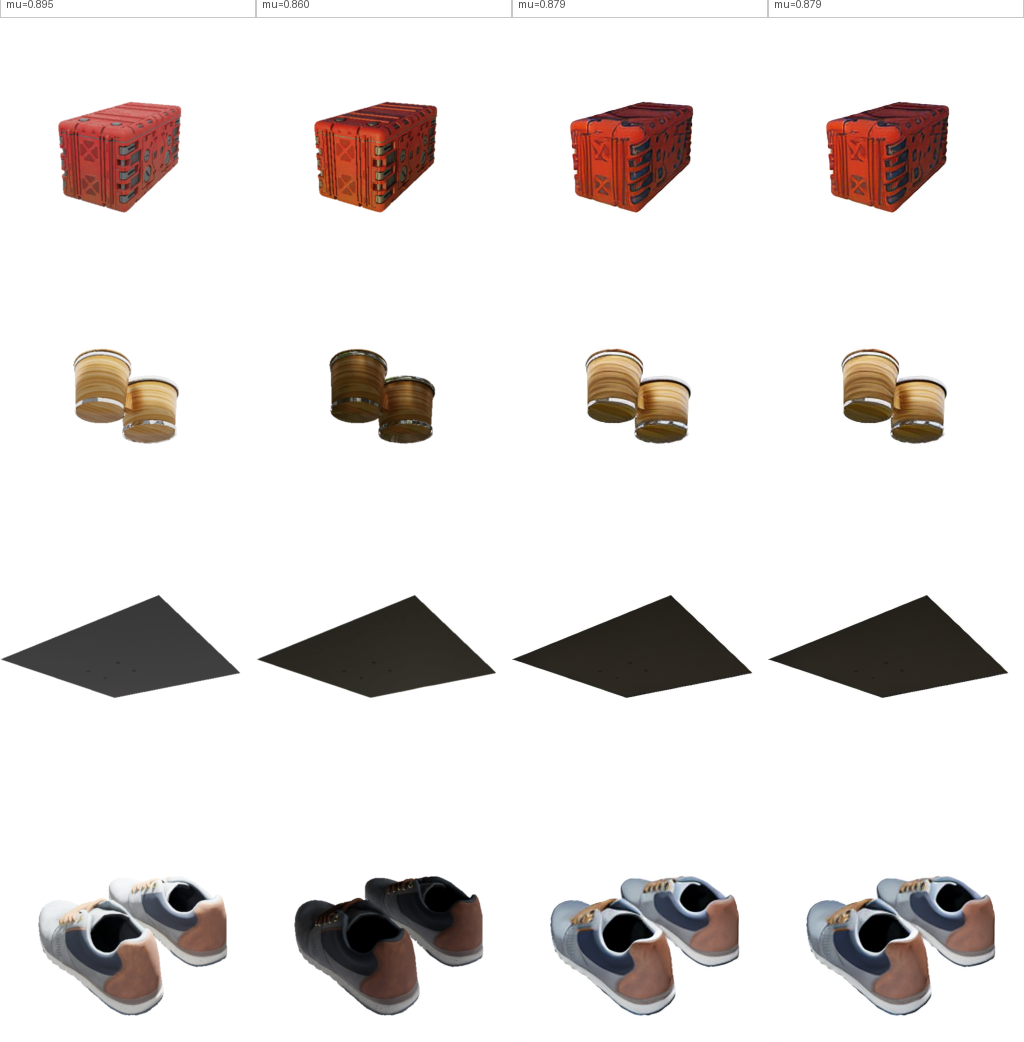
\includegraphics[width=\linewidth]{problem_def_ra_failure_result.png}
\caption{失败结果区}
\end{subfigure}\hfill
\begin{subfigure}{0.28\linewidth}
\centering
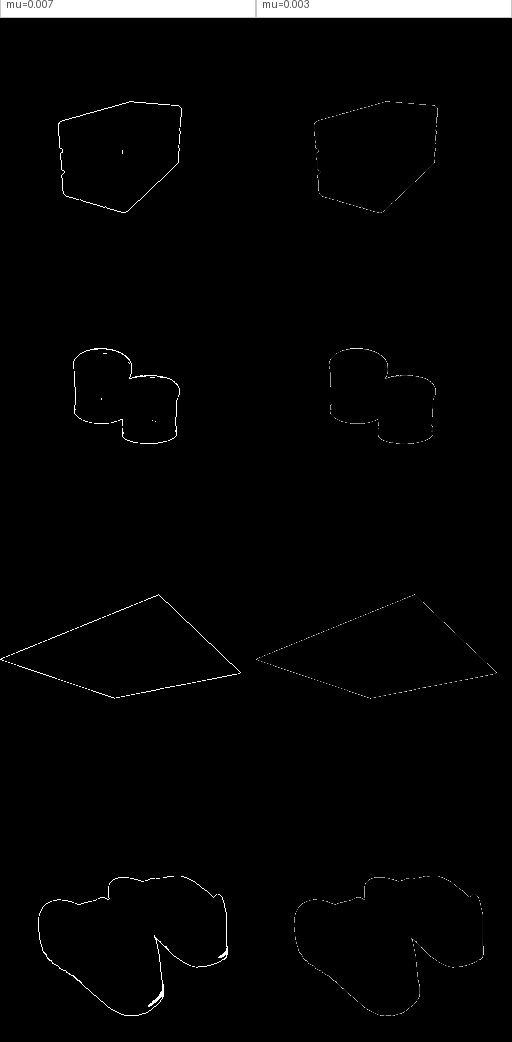
\includegraphics[width=\linewidth]{problem_def_ra_failure_diagnostic.png}
\caption{对应诊断区域}
\end{subfigure}
\caption{失败案例图。当前方法虽然能够显著提升高光监督稳定性，但在部分极端随机面光源样例中，仍可能出现对宽波瓣高光支持不足的问题。}
\label{fig:failure_case_cn}
\end{figure}

\section{结果呈现计划}

本文实验部分建议分三层呈现：

\begin{enumerate}
\item 基于当前仓库已有 run 的“证据对齐版”消融表；
\item 补齐缺失实验后的“最终 clean ablation 表”；
\item 单独的效率章节，用于展示 hybrid 与 pure latent probe 的效果-效率权衡。
\end{enumerate}

在图示排版上，每个对比样例建议至少包含输入图、目标光照、GT、baseline、本文方法与局部放大高光区域。由于 \texttt{ra} 划分最能暴露本文关注的 failure mode，因此应优先用于主图展示。

\section{当前实验状态}

基于当前仓库已有 run，可作如下阶段性判断：

\begin{enumerate}
\item \texttt{jbhdfvfc} 是当前主 held-out 最强的 run，可作为主方法锚点。
\item \texttt{spuru5qy} 是当前最均衡的 run，尤其适合突出随机面光源鲁棒性。
\item \texttt{fi04f78e} 是当前最适合解释 local-relative highlight 定义的 run。
\item \texttt{xkmlb19f} 与 \texttt{iepfybfu} 更适合作为效率侧证据，而不是主方法核心证据。
\end{enumerate}

明确区分这些 run 的角色，有助于论文写作时避免把“主方法效果”与“效率变体效果”混为一谈。

\section{当前初稿写作口径}

基于现有实验与图示准备情况，当前中文初稿建议采用如下写法：

\begin{enumerate}
\item 在方法部分，将前景优先、分位数阈值、blur-only threshold estimation 与 local-relative highlight 组织为一个统一的方法故事，而不是拆成彼此独立的小技巧。
\item 在实验部分，明确声明主方法消融表目前是“证据对齐版”而非最终 clean ablation，以保证论文口径诚实且可持续扩展。
\item 在定性部分，优先展示 \texttt{ra} 样例以突出 failure mode，再用 \texttt{uu} 与 \texttt{us} 样例证明主 held-out 结果并未牺牲。
\item 在效率部分，将 hybrid probe distillation 与 pure latent replacement 单列，强调其角色是效果-效率权衡，而不是主方法替代。
\end{enumerate}

\section{讨论与局限}

本文方法在不增加推理复杂度的前提下稳定了高光监督，因此具有较强工程实用性。但从当前实验与相关工作比较来看，其仍存在若干局限：

\begin{enumerate}
\item 方法仍然依赖显式前景 mask 或较可靠的回退前景估计；
\item 相对高光引导虽然提升了稳定性，但在极端材质与极端光照条件下仍无法完全消除歧义；
\item 当前工作主要聚焦监督设计，而非显式物理分解，因此在理论上仍不具备严格的光传输一致性；
\item 更大规模结构改造、显式 specular-diffuse 分解、阴影与高光联合建模，以及更强的多光照条件建模仍有待进一步研究。
\end{enumerate}

\section{结论}

本文针对扩散式物体重光照在镜面材质与面光源条件下高光监督不稳定的问题，提出了一种前景掩码感知的相对高光引导框架。该框架通过前景优先掩码、局部相对高光定义、前景内分位数阈值、仅用于阈值估计的模糊以及图像空间高光辅助监督，共同提高了高光监督的稳定性与可解释性。现有结果表明，所提方法在主 held-out 设置上取得了稳定增益，并在随机面光源划分上表现出更强鲁棒性。进一步地，本文还通过 hybrid probe distillation 与 pure latent replacement 的对比，展示了图像空间高光分支在效果-效率权衡中的关键作用。后续工作将围绕 clean ablation、跨域实验与更规范的图示排版继续完善，从而形成完整的投稿版本。

\section*{作者信息}

\noindent 作者甲，出生年份，职称或身份，研究方向，E-mail: \href{mailto:author1@example.com}{author1@example.com}

\noindent 作者乙，出生年份，职称或身份，研究方向，E-mail: \href{mailto:author2@example.com}{author2@example.com}

\begin{thebibliography}{99}

\bibitem{ref_ng}
Jin H, Li Y, Luan F, Xiangli Y, Bi S, Zhang K, Xu Z, Sun J, Snavely N. Neural Gaffer: Relighting Any Object via Diffusion[EB/OL]. arXiv:2406.07520, 2024.

\bibitem{ref_lightit}
Kocsis P, Philip J, Sunkavalli K, Nie{\ss}ner M, Hold-Geoffroy Y. LightIt: Illumination Modeling and Control for Diffusion Models[C]//Proceedings of the IEEE/CVF Conference on Computer Vision and Pattern Recognition. 2024: 9359--9369.

\bibitem{ref_spotlight}
Fortier-Chouinard F, Zhang Z, Messier L E, Garon M, Bhattad A, Lalonde J F. SpotLight: Shadow-Guided Object Relighting via Diffusion[EB/OL]. arXiv:2411.18665, 2024.

\bibitem{ref_illuminerf}
Zhao X, Sargent K, Luo D, Ren Y, Bhat S F, Srinivasan P P. IllumiNeRF: 3D Relighting Without Inverse Rendering[EB/OL]. arXiv:2406.06527, 2024.

\bibitem{ref_lightrig}
He Z, Wang T, Huang X, Pan X, Liu Z. Neural LightRig: Unlocking Accurate Object Normal and Material Estimation with Multi-Light Diffusion[EB/OL]. arXiv:2412.09593, 2024.

\end{thebibliography}

\end{document}
